%! Author = phili
%! Date = 25/06/2021

\section{Threat Modeling}
\subsection{Securing DevOps}
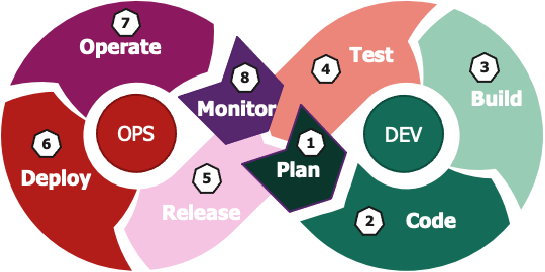
\includegraphics[width=0.5\linewidth]{../img/devops_infinity.png}
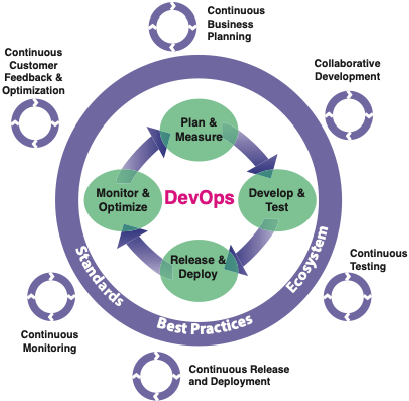
\includegraphics[width=0.5\linewidth]{../img/devops_reference_architecture.png}

\subsection{Four Major Activities}
\begin{itemize}
    \item Plan and measure
    \item Develop and test
    \item Release and deploy
    \item Monitor and optimize
\end{itemize}

\subsection{Continous Secutity}
\begin{itemize}
    \item Prepare the organisation
    \item Protect the software
    \item Produce well secured software
    \item Respond to vulnerabilities
\end{itemize}

\subsection{Security in the Phases}
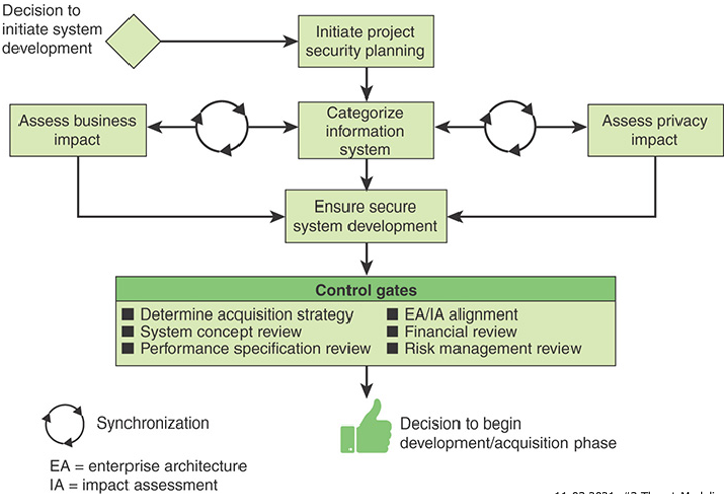
\includegraphics[width=\linewidth]{../img/security_in_phases.png}
\textbf{Major Security Activities:} A number of
security-related activities are needed to assure
that security is incorporated effectively in that
design phase\\
\textbf{Expected Outputs:} A key to success is to
define specific deliverables for each activity\\
\textbf{Synchronization:} A feedback loop between
tasks provides opportunities to ensure that the
SDLC is implemented as a flexible approach
that allows for appropriate and consistent
communication and the adaptation of tasks and
deliverables as the system is developed\\
\textbf{Control gates:} Decision points at the end of
each phase when the system is evaluated and
management determines whether the project
should continue as is, change direction, or be
discontinued\\

\subsubsection{Initiate project security planning}
\begin{itemize}
    \item Identify key security roles
    \item Identify the standards and regulations for the system
    \item Develop an overall plan for security milestones
    \item Get Stakeholders to have a common understanding (security implications, considerations, requirements)
    \item Enable developers to design security features
    \item \textbf{Output:} Supporting documents of all decisions
\end{itemize}

\subsubsection{Categorize information system}
\begin{itemize}
    \item Identify information that will be transmitted, processed or stored
    \item Define applicable levels of information categorization (based on impact analysis)
    \item \textbf{Result:} Catalog of information types
    \item \textbf{Outputs:} Definitions of categories, level of effort estimate
\end{itemize}

\subsubsection{Ensuring secure system development}
\begin{itemize}
    \item Develop a set of principles of security expectations
    \begin{itemize}
        \item Secure concept of operations
        \item Standards and processes
        \item Security training for development team
        \item Quality management
        \item Secure environment
        \item Secure code practices and repositories
    \end{itemize}
    \item \textbf{Output:} Plans for development security training / quality assurance
\end{itemize}

\subsubsection{Control Gates}
\begin{itemize}
    \item Determine acquisition strategy
    \item System concept review
    \item Performance specification review
    \item EA/IA alignment
    \item Financial review
    \item Risk management review
\end{itemize}

\subsection{Develop \& Test}
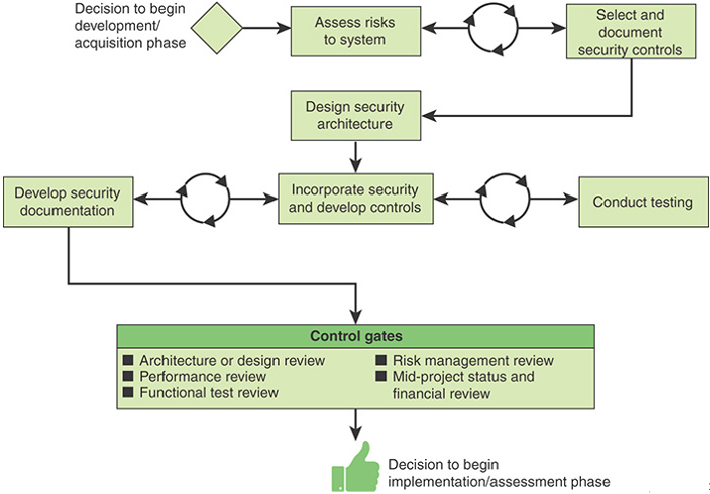
\includegraphics[width=\linewidth]{../img/develop_and_test.png}

\subsubsection{Designing the security architecture}
\begin{itemize}
    \item Produce a detailed architecture
    \item Incorporate security features and controls into the system design
    \item \textbf{Outputs:} 
    \begin{itemize}
        \item Schematic of security integration
        \item List of shared services
        \item Identification of common controls used by the system
    \end{itemize}
\end{itemize}

\subsubsection{Control Gates}
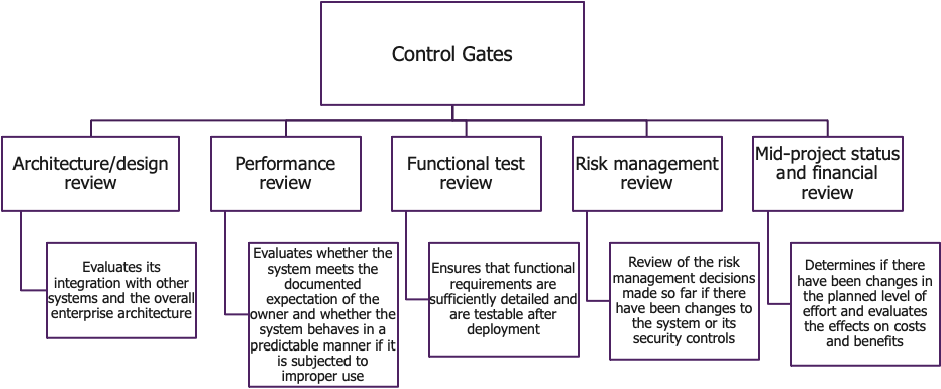
\includegraphics[width=\linewidth]{../img/control_gates.png}

\subsubsection{Begin Implementation / Assessment phase}
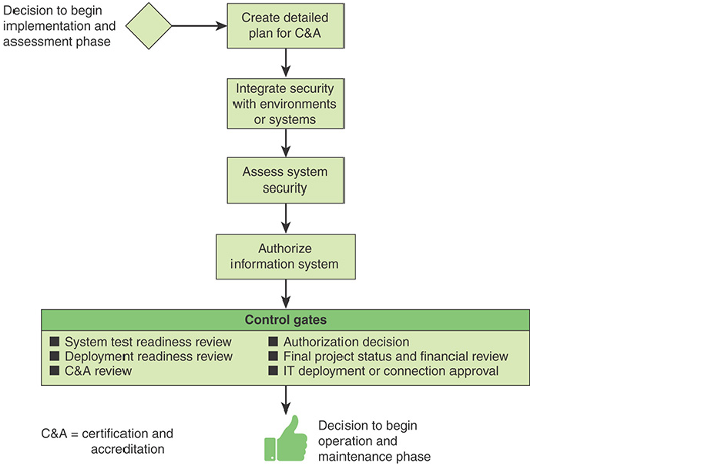
\includegraphics[width=\linewidth]{../img/develop_and_test2.png}

\subsubsection{Control Gates}
\begin{itemize}
    \item System test readiness review
    \item Deployment readiness review
    \item Certification and accreditation review
    \item Authorization decision
    \item Final project status and financial review
    \item IT deployment or connection approval
\end{itemize}

\subsubsection{Begin Operations and Maintenance phase}
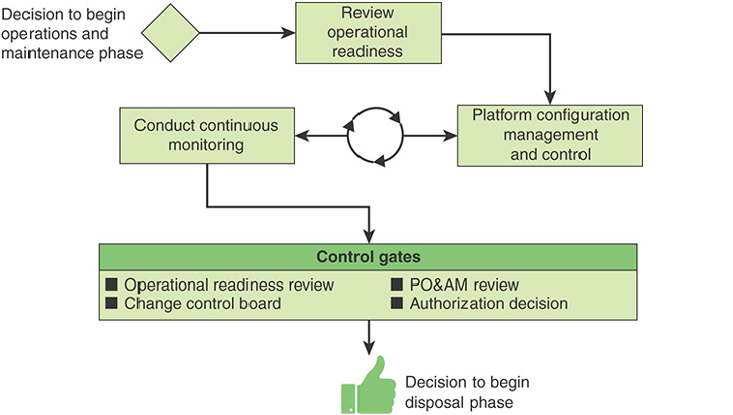
\includegraphics[width=\linewidth]{../img/develop_and_test3.png}

\subsubsection{Initiate disposal phase}
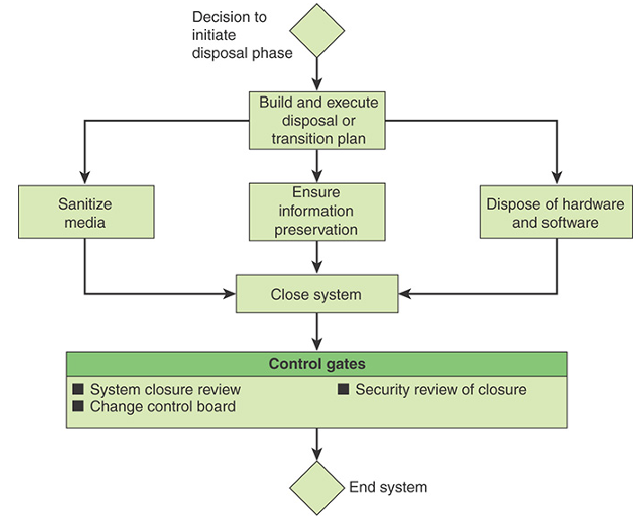
\includegraphics[width=\linewidth]{../img/develop_and_test4.png}

\subsection{Continous Security}
\begin{enumerate}
    \item Test driven Security
    \item Monitor and respond to attacks
    \item Assess risks and mature security
\end{enumerate}

\subsection{Risk Management}
\subsubsection{Activities}
\textbf{Summary:}\\
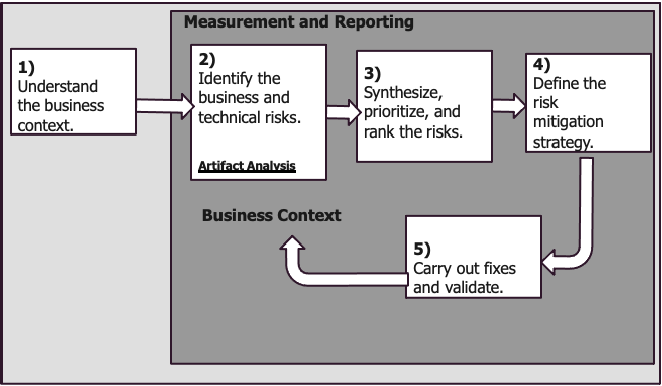
\includegraphics[width=\linewidth]{../img/risk_management_activities.png}
\begin{enumerate}
    \item Understand the business context
    \begin{itemize}
        \item Extract and describe business goals
        \item Set prios
        \item Understanding what risks to consider
        \item Gathering the artifacts
        \item Conducting project research to the scope
    \end{itemize}
    \item Identifying the business and technical risks (priorize / rank)
    \begin{itemize}
        \item Business risks impact business goals
        \item Map technical risks to business goals
        \item Develop a set of risk questionnaires
        \item Interview the target project team
        \item Analyse the research interview data
        \item Evaluate software artifacts
    \end{itemize}
    \item Synthesize, prioritize and rank the risks
    \begin{itemize}
        \item Prio the risks based on business goals
        \item Apply risk metrics
        \item Number of risks emerging over time
        \item What shall be done first?
        \item What is the best allocation of resources?
    \end{itemize}
    \item Define the risk mitigation strategy
    \begin{itemize}
        \item Take into account: Cost, Implementation time, Likelihood of success, Competence and impact
        \item Identify the validation techniques
        \item Metrics are financial in nature
    \end{itemize}
    \item Carry out fixes and validate their correctness
    \begin{itemize}
        \item Implement the mitigation strategy
        \item Rectify artifacts
    \end{itemize}
\end{enumerate}

\subsubsection{Summary}
\begin{itemize}
    \item Relies on continuous and consistent identification of risks.
    \item The five fundamentals should be applied repeatedly
    \item Use project management tools to track risk information
\end{itemize}

\subsection{Attack Trees}
\begin{itemize}
    \item Tree-structured graph
    \item Showing how a system can be attacked
\end{itemize}
\textbf{Construction:}
\begin{enumerate}
    \item Identify goals (1 Tree per goal)
    \item Identify attacks against goals
    \item Existing sub-trees can be plugged in
\end{enumerate}
\textbf{Usage:}
\begin{itemize}
    \item Propagate up the tree
    \item You can specify values that represent other different meanings (Equipment / Cost)
    \item Combine Node Values
\end{itemize}

\subsubsection{Example}
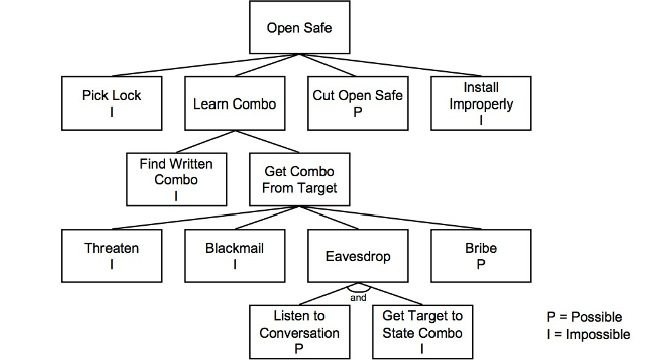
\includegraphics[width=\linewidth]{../img/attack_tree_example.png}
\textbf{Countermeasures:}\\ 
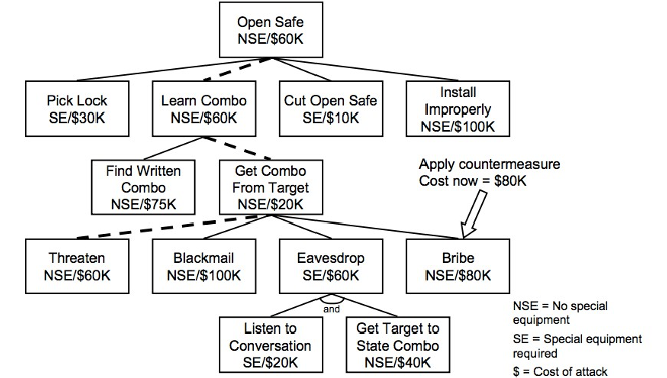
\includegraphics[width=\linewidth]{../img/attack_tree_example2.png}
